% !TeX spellcheck = en_US
% !TeX encoding = UTF-8

\documentclass[
	paper=A4,
	twoside=true,
	openright,
	parskip=full,
	chapterprefix=true,
	11pt,
	headings=normal,
	bibliography=totoc,
	listof=totoc,
	titlepage=on,
%	draft
	final
	]{scrreprt}

\usepackage{lieb}
\graphicspath{{images/}}

\title{Development of a Fast Search Algorithm for the MUSiC Framework}
\date{09.09.2015}
\author{Jonas Lieb}

\makeatletter
\let\theauthor\@author
\let\thetitle\@title
\makeatother

\hypersetup{
	pdftex,
	pdfauthor={\theauthor},
	pdftitle={\thetitle},
	pdflang={en-US},
}

\begin{document}

\cleardoublepage
\pagenumbering{roman}
\pagestyle{empty}

\makeatletter
\begin{titlepage}
\begin{center}

\vspace{30mm}

\Huge \@title

\vspace{30mm}

\normalsize von \\

\vspace{5mm}

\LARGE \@author

\vspace{30mm}

\Large Bachelorarbeit im Fach Physik \\ \vspace{5mm}
\normalsize vorlegegt der \\
\Large Fakultät für Mathematik, Informatik und Naturwissenschaften \\
der RWTH Aachen \\ \vspace{5mm}
\normalsize im \\ \Large Juli 2015 \\ \vspace{5mm}
\normalsize angefertigt am \\ \Large III. Physikalischen Institut (IIIA) \\ \vspace{5mm}
\normalsize bei \\ \Large Prof. Dr. Thomas Hebbeker \vspace{5mm}

\end{center}
\end{titlepage}
\makeatother
\cleardoublepage
% !TeX spellcheck = de_DE
% !TeX encoding = UTF-8
% !TeX root = ../document.tex

Ich versichere, dass ich die Arbeit selbständig verfasst und keine anderen als die angegebenen Quellen und Hilfsmittel benutzt sowie Zitate kenntlich gemacht habe.

Aachen, den \todo{Datum}
\cleardoublepage

% !TeX spellcheck = en_US
% !TeX encoding = UTF-8
% !TeX root = ../document.tex

\chapter*{Abstract}
The CMS experiment at the LHC produces a vast amount of data: each second about \SI{20}{\tera\byte} of information is generated by the detector hardware. Naturally, the analysis also requires a lot of computing power. Using a chain of several algorithms the detector signal is interpreted as physical meaningful data, on which state of the art analyses are performed. 

The Model Unspecific Search in CMS (MUSiC) is an analysis that performs on a wide spectrum of final states. Kinematic distributions of these final states are aggregated and compared to the expectation from Monte Carlo simulations. By searching for deviations, MUSiC is sensitive to indications of physics beyond the standard model.

This thesis proposes, implements and validates an additional step in the MUSiC analysis, which drastically improves computing performance.

% !TeX spellcheck = de_DE
% !TeX encoding = UTF-8
% !TeX root = ../document.tex

\vspace*{5mm}
\vspace*{\fill}
{\usekomafont{chapter}Kurzdarstellung}
\chapterheadendvskip

Das CMS Experiment am LHC produziert sehr große Datenmengen: pro Sekunde werden rund \SI{20}{\tera\byte} an Daten von der Detektorhardware generiert. Selbstverständlich erfordert die Auswertung viel Rechenleistung. Mithilfe mehrerer Algorithmen wird dem Detektorsignal eine physikalische Bedeutung zugewiesen, aufgrund derer modernste Analysen durchgeführt werden.

Die modellunspezifische Suche MUSiC (engl: Model Unspecific Search in CMS) ist eine Analyse, die auf einem breiten Spektrum von Endzuständen arbeitet. Dabei werden kinematische Verteilungen der Endzustände erstellt und mit Erwartungen aus Monte-Carlo-Simulationen verglichen. Die Suche nach Abweichungen macht MUSiC sensitiv gegenüber Anzeichen von Physik jenseits des Standardmodelles.

Diese Arbeit erklärt, implementiert und validiert einen zusätzlichen Arbeitsschritt der MUSiC-Analyse, der die Rechenzeit drastisch reduziert.
\cleardoublepage

\tableofcontents

\cleardoublepage
\pagenumbering{arabic}
\setcounter{page}{1}
\pagestyle{maincontentstyle}

% !TeX spellcheck = en_US
\chapter{Introduction}

\section{Units and Notation}
Throughout this work, a subset of the natural unit system will be used, as it is convention in high energy particle physics. The speed of light and the reduced Planck constant are fixed to $c = 1$ and $\hbar = 1$, and as such they are omitted in equations. Additionally, energy is expressed in \eV, where \unit{1}{\eV} is the energy gain of an electron which is accelerated across a \unit{1}{\volt} potential ($\unit{1}{\eV} \approx \unit{1.602 \e{-19}}{\joule}$). These conventions induce a change in units for the other dimensions, most importantly mass and momentum, both of which are notated in \eV.

\section{The Standard Model}
The \emph{standard model} (SM) is a theory that represents our current knowledge of elementary particles, their forces and interactions, excluding gravity. 

Particles in the standard model can be classified into two separate classes: \emph{Fermions}, which make up matter and possess a spin of \nicefrac{1}{2}, and \emph{bosons}, which are mediators of forces and possess an integer spin.
Three elementary forces are predicted: \emph{electrodynamic} (Quantum Electrodynamics, QED), \emph{strong} (Quantum Chromo Dynamics, QCD) and \emph{weak} (Quantum Flavor Dynamics). The forces are induced by corresponding charge-like properties: electrodynamic charge, color charge and weak isospin. These charges can then be used to further subdivide fermions into \emph{quarks} and \emph{leptons}, which will be described in the following sections. 

The standard model also provides theoretical predictions about the relations between particles, their masses and the probabilities of certain processes to happen. Because the probability is proportional to the number of times that a process occurs, experimentalists can validate the standard model by counting events with certain outcomes.

\subsection{Leptons}
There are three charged leptons: the \emph{electron} (\Pe), the \emph{muon} (\Pmu) and the \emph{tau} (\Ptau). They carry the electric charge of \unit{-1}{e} and participate in electrodynamic and weak interactions. For each charged lepton, there is one \emph{neutrino} counterpart (\Pnue, \Pnum, \Pnut). Neutrinos are electrically neutral, weakly interacting, massless particles. They remain undetected in current collider detectors.
The leptons do not carry color charge and are thus excluded from the strong interaction.
An overview about the leptons and their masses can be found in table~\ref{tbl:sm_leptons}.

\begin{table}[htbp]
	\center
	\begin{tabular}{ r | l | l | l | }
		\cline{2-4}
		& \multicolumn{3}{c|}{Leptons} \\ \cline{2-4}
		& electron (\Pe) & muon (\Pmu) & tau (\Ptau) \\ \cline{2-4}
		mass & \unit{511.0}{\keV} & \unit{105.7}{\MeV} & \unit{1.777}{\GeV} \\ \cline{2-4}
		charge & $-1$ & $-1$ & $-1$ \\ \cline{2-4}
		& \Pe neutrino (\Pnue) & \Pmu neutrino (\Pnum) & \Ptau neutrino (\Pnut) \\ \cline{2-4}
		mass & $< \unit{2}{\eV}$ & $< \unit{0.19}{\MeV}$ & $< \unit{18.2}{\MeV}$ \\ \cline{2-4}
		charge & 0 & 0 & 0 \\ \cline{2-4}
	\end{tabular}
	\caption{Leptons in the standard model\cite[p.~30, p.~690f.]{Oo2014Review}.}
	\label{tbl:sm_leptons}
\end{table}

\subsection{Quarks}
Similarly to the leptons, quarks can be divided into three generations. The first generation contains the stable \emph{up} and \emph{down} quarks, the second generation the \emph{charm} and \emph{strange} quarks and the third generation contains the heavy \emph{top} and \emph{bottom} quarks. Quarks carry a fractional electric charge of either \unit{\nicefrac{2}{3}}{e} or \unit{\nicefrac{-1}{3}}{e}.
They also carry color charges and take part in the strong interaction as well as in the weak interaction.
The three quark generations and their properties are shown in table~\ref{tbl:sm_quarks}.

\begin{table}[htbp]
	\center
	\begin{tabular}{ r | l | l | l | }
		\cline{2-4}
		& \multicolumn{3}{c|}{Quarks} \\ \cline{2-4} 
		& up (\Pup) & charm (\Pcharm) & top (\Ptop) \\ \cline{2-4}
		mass & \unit{2.3}{\MeV} & \unit{1.28}{\GeV} & \unit{173.2}{\GeV} \\ \cline{2-4}
		charge & \nicefrac{2}{3} & \nicefrac{2}{3} & \nicefrac{2}{3} \\ \cline{2-4}
		& down (\Pdown) & strange (\Pstrange) & bottom (\Pbottom) \\ \cline{2-4}
		mass & \unit{4.8}{\MeV} & \unit{95}{\MeV} & \unit{4}{\GeV} \\ \cline{2-4}
		charge & \nicefrac{-1}{3} & \nicefrac{-1}{3} & \nicefrac{-1}{3} \\ \cline{2-4}
	\end{tabular}
	\caption{Quarks in the standard model\cite[p.~33]{Oo2014Review}.}
	\label{tbl:sm_quarks}
\end{table}

\subsection{Bosons}
Gauge bosons are mediators of the elementary forces. QED is mediated by the massless \emph{photon} (\Pphoton), QCD by the massless \emph{gluon} (\Pgluon) and the weak interaction by the massive \PZ and \PWpm bosons. They couple to the corresponding charges. To account for the massive boson masses, the Higgs mechanism is introduced. The Higgs field gives rise to the Higgs boson (\PHiggs), a candidate of which has been found in 2012\cite{Ao2015Combined}.
All bosons and their properties are listed in table \ref{tbl:sm_bosons}.

\begin{table}[htbp]
	\center
	\begin{tabular}{ r | l | l | l | l | l |}
		\cline{2-6}
		& \multicolumn{5}{c|}{Bosons} \\ \cline{2-6} 
		& Photon (\Pgamma) & Gluon (\Pgluon) & Z-Boson (\PZ) & W-Bosons (\PWpm) & Higgs (\PHiggs) \\ \cline{2-6}
		mass & 0 & 0 & \unit{91.2}{\GeV} & \unit{80.4}{\GeV} & \unit{126}{\GeV} \\ \cline{2-6}
		charge & 0 & 0 & 0 & $\pm 1$ & 0 \\ \cline{2-6}
		interaction & QED & QCD & weak & weak & Higgs \\ \cline{2-6}
	\end{tabular}
	\caption{Bosons in the standard model\cite[p.~27]{Oo2014Review}.}
	\label{tbl:sm_bosons}
\end{table}

\subsection{Antiparticles}
For each SM particle, there exists one counterpart with the same mass but an opposite sign for all charge-like properties, called \emph{antiparticle}. Unlike fermions, bosons are their own antiparticles, called Majorana particles.

\section{The Large Hadron Collider}
Elementary particles and the standard model are commonly studied using scattering experiments. Two options arise: \emph{fixed target} and \emph{collider} experiments. Latter ones are preferred for high energies due to kinematic reasons.
A collider can be separated into two basic parts: an \emph{accelerator} and a \emph{detector}.
Inside the accelerator, the particles are accelerated to high energies using an electric field on a circular trajectory, which is enforced by dipole magnets. Two beams are maintained, circulating in opposite directions, which are deflected inside the detectors positioned along the ring to produce collisions.

\begin{figure}[htbp]
	\center
	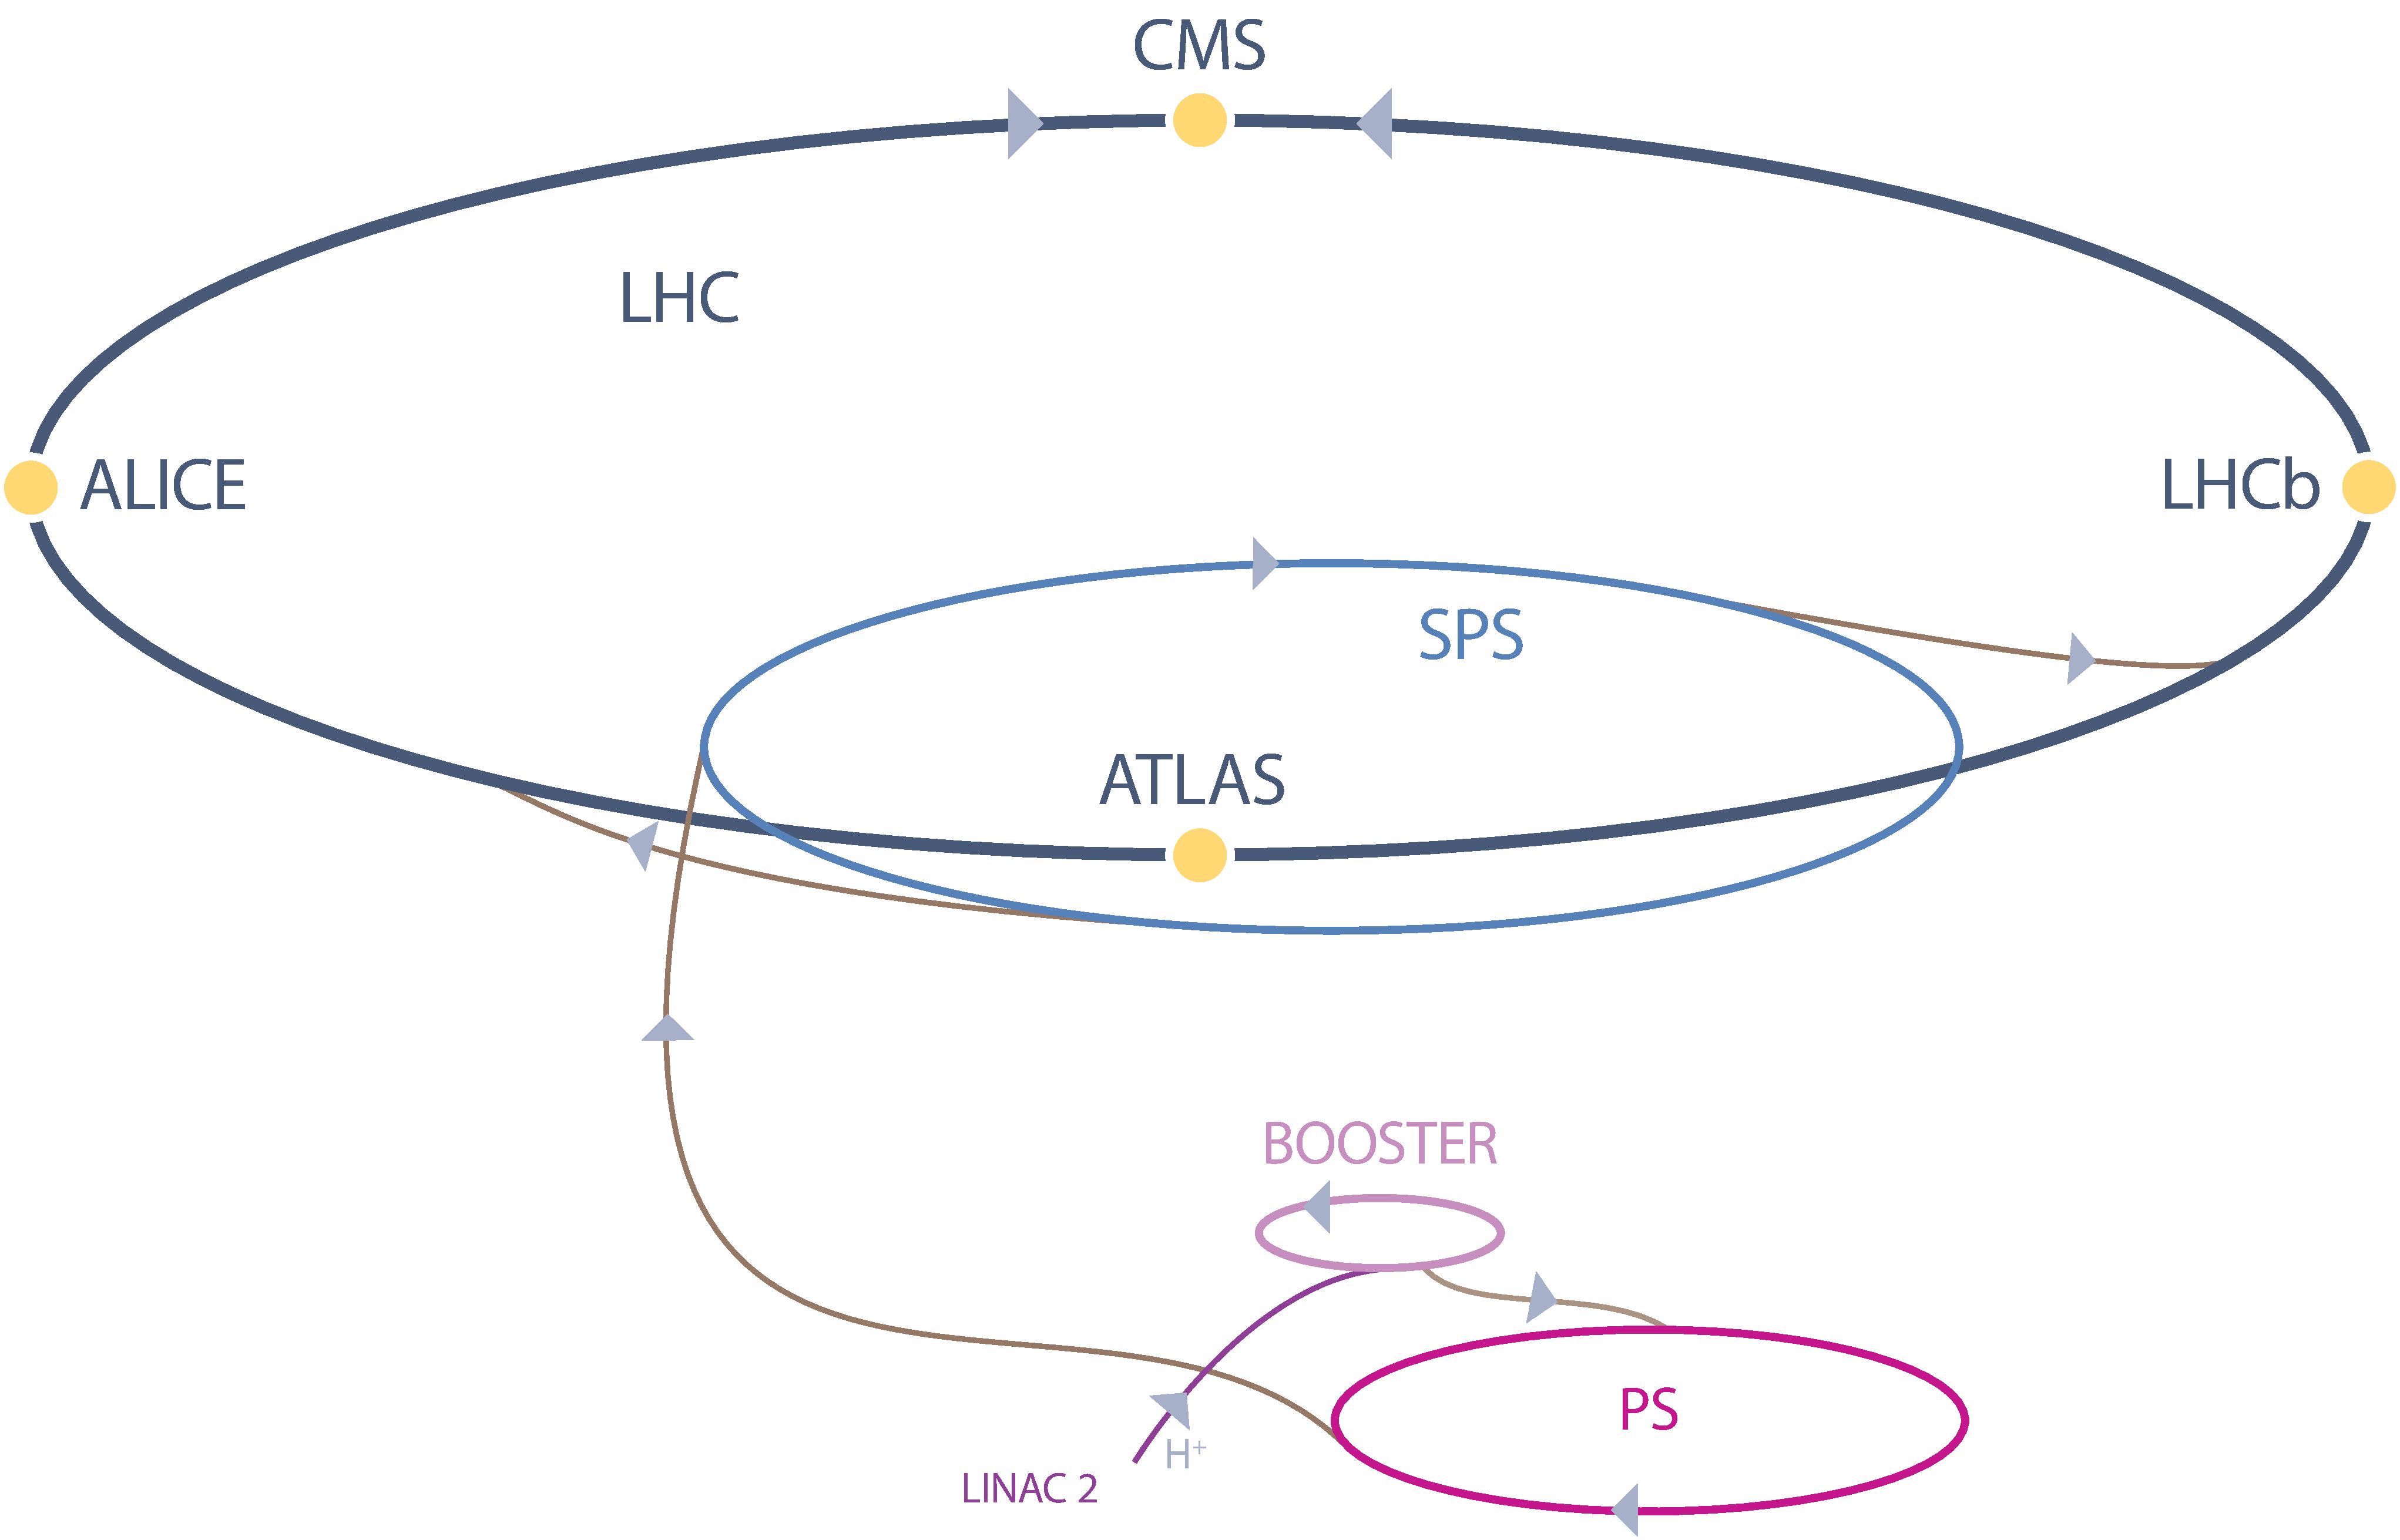
\includegraphics[width=0.5\textwidth]{CERN_accelerator_complex.pdf}
	\caption{The CERN accelerator complex\cite[modified]{Marcastel2013CERNs}. Shown are the LHC ring, the preaccelerators (Linear Accelerator 2, BOOSTER, Proton Synchrotron, Super Proton Synchrotron) and the four LHC experiments: CMS, ATLAS, ALICE and LHCb.}
	\label{fig:cern_accelerator_complex}
\end{figure}

The \emph{Large Hadron Collider} (LHC) is a proton-proton collider experiment of the European Organization for Nuclear Research (\emph{Conseil Européen pour la Recherche Nucléaire}, CERN), situated between \unit{45}{\meter} and \unit{170}{\meter} underground near Geneva, Switzerland. The LHC has been installed in the tunnel of the former LEP collider, having a circumference of \unit{26.7}{\kilo\meter}\cite{BV2009CERN,EB2008LHC}. The proton beams are injected after passing a series of preaccelerators, as shown in figure \ref{fig:cern_accelerator_complex}. It has been designed to provide an energy of \unit{7}{\TeV} per beam, resulting in a center-of-mass energy $\sqrt{s} = \unit{14}{\TeV}$. It is currently (2015) running at $\sqrt{s} = \unit{13}{\TeV}$, the data analyzed in this work were taken in 2012 with $\sqrt{s} = \unit{8}{\TeV}$.

\section{The Compact Muon Solenoid detector}
CMS is an experiment at the LHC. The CMS detector consist of a barrel section along the beam pipe, which is closed off by two end caps. Collisions happen in the center of the barrel at the interaction point. 
The detector parts and particle footprints can be found in figure \ref{fig:cms_slice}.
Close to the \emph{interaction point}, the inner part of the barrel contains a \emph{silicon tracker} used to record trajectories of charged particles. 
The inner tracker is surrounded by an \emph{electromagnetic calorimeter} (ECAL) made of lead tungstate crystals. The ECAL measures energy deposited by electrons and photons, combined with the tracker it can distinguish between the two particle types. 
After the electromagnetic calorimeter follows the \emph{hadron calorimeter} (HCAL). It is a sampling calorimeter composed of layers of brass absorber plates and plastic scintillator fibers. Due to the high density of the brass absorbers, hadronic showers deposit most of their energy inside the HCAL.
The HCAL is surrounded by the most important feature of the CMS detector, the \emph{solenoid magnet}. The solenoid coil is cooled down below \unit{10}{\kelvin}, where the NbTi (Niobium-Titanium) conductor becomes superconducting, allowing for currents up to \unit{19}{\kilo\ampere}. The resulting field strength in the center of the coil is \unit{4}{\tesla}. The strong magnetic field causes the particle tracks to bend, this effect is used to measure the momentum of particles.
In the outer part one finds the iron return yoke interspersed with \emph{muon drift chambers}. Since only muons and neutrinos pass through the solenoid and iron yoke and neutrinos remain undetected, the drift chambers can precisely assess the muon momentum.\cite{Co2008CMS}

\begin{figure}[htbp]
	\center
	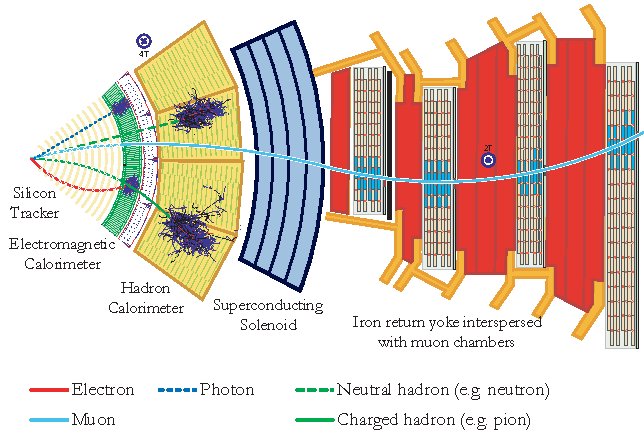
\includegraphics[width=\textwidth]{CMS_Slice.pdf}
	\caption{Slice through the CMS detector. The different detector layers (tracker, ECAL, HCAL, magnet, muon chambers) are shown, alongside schematic tracks of an electron, a photon, a charged and neutral hadron and a muon.\cite[modified]{Barney2011CMS}}
	\label{fig:cms_slice}
\end{figure}

\subsection{Coordinate System}
The CMS collaboration has defined a spherical coordinate system inside the detector, as illustrated in figure \ref{fig:cms_coordinate_system}. The origin is located in the interaction point, the z-axis points along the beam pipe towards the Jura mountains. The x-axis is defined towards the center of the LHC ring. An azimuthal angle $\phi$ is defined from the x-axis in the x-y plane. The polar angle $\theta$ is measured from the z-axis. One can also define a radial coordinate $r$ in the x-y plane, as distance from the z-axis.\cite[p. 2]{Co2008CMS} 

\begin{figure}[htbp]
	\center
	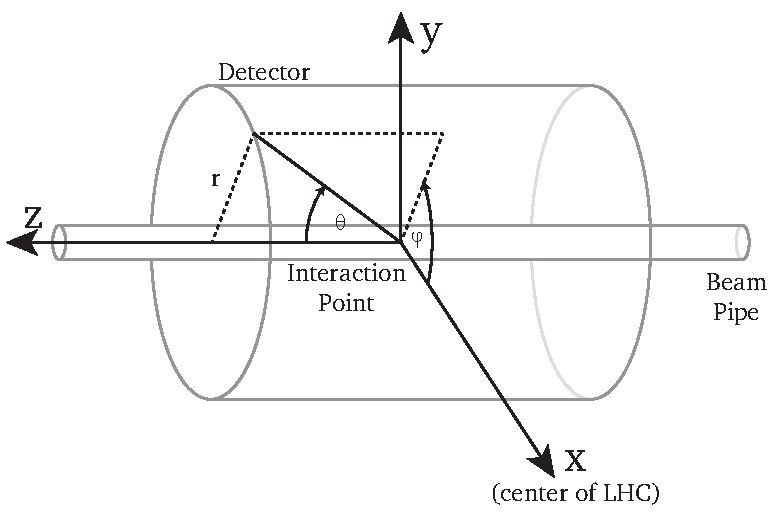
\includegraphics[width=0.9\textwidth]{CMS_coordinate_system.pdf}
	\caption{The CMS coordinate system.}
	\label{fig:cms_coordinate_system}
\end{figure}

\section{Commonly used quantities}
Since the particles initially move along the z-axis and only scatter partially, the exact longitudinal velocity of the center-of-momentum frame is unknown. 
Thus, most of the kinetic variables are defined in the transverse (x-y) plane. A particle is assigned a \emph{transverse momentum} \pT which only contains the transverse component of its momentum vector. Analogous, only a fraction of the energy is regarded, the \emph{transverse energy} \ET. 
The sum of all transverse momenta in a final state is usually not equals to zero, since invisible neutrinos carry away some of the momentum. This is accounted for by the negative sum of the transverse energy, which is called \emph{missing transverse energy} \MET.
Another commonly used quantity is the pseudo-rapidity $\eta = -\ln \tan(\theta/2)$, which has the property that its distances are Lorentz invariant.

\section{Bunch crossings, events, collisions and pileup}
For practical acceleration purposes, the protons circulating in the LHC beam pipe are grouped into 2808 \emph{bunches}\cite[p.4]{EB2008LHC}. A \emph{bunch crossing} happens every \unit{50}{\nano\second} (2012), defining an \emph{event}. During an event, any number of hard collisions can occur. Events with multiple pp-collisions are called \emph{pileup} events.

\section{Trigger}
Since the raw data for each event is about $\order{\unit{1}{\mega\byte}}$, the throughput required to transfer all data would be $\order{\unit{20}{\tera\byte}}$ per second. This amount of data is too much for current hard- and software, thus a selection mechanism is introduced to match the amount of recorded data to the networking, processing and storage capabilities. This system is called \emph{trigger}. The CMS trigger system consists of two layers, the "Level-1 Trigger" (L1), implemented in hardware on site, and the software "High-Level-Trigger" (HLT), located at a computing farm close to the detector. For each run, the operator defines a set of selection requirements, called \emph{trigger menu}. These requirements reduce the data amount by $\order{10^{-6}}$.

\section{Event reconstruction}
In the \emph{reconstruction} (RECO) step, various algorithms are executed offline to reconstruct physics objects from the recorded data. The most important inputs are the bending radius of the particle tracks, energy deposits in the calorimeters and hits in the muon chambers. 
A notable algorithm that ensures that each input is linked to exactly one physics object has been developed by CMS and is called \emph{Particle-Flow}\cite{2009Particle}. 
% !TeX spellcheck = en_US
% !TeX encoding = UTF-8
% !TeX root = ../document.tex

\chapter{Model Unspecific Search in CMS}

The Model Unspecific Search in CMS (\emph{MUSiC})\cite{Pieta2012MUSiC,Papacz2014Model,Duchardt2015MUSiC} is an analysis procedure that compares observed data to the standard model expectation from Monte Carlo (MC) simulations. Unlike dedicated analyses that usually only regard a few final states, an unspecific search covers a broad spectrum of final states.
This is especially useful since some theories predict small deviations in many final states, which on their own would not be classified as significant, but in total have a scientific impact.

This chapter will focus on the MUSiC workflow. First, the motivation behind an unspecific search will be illustrated, then the three analysis steps \emph{skimming}, \emph{classification} and \emph{scanning} will be explained.

\section{Motivation}
Since a Higgs boson candidate has been discovered at the LHC\cite{Ao2015Combined}, all predicted SM particles have been observed.
Nevertheless there are many unsolved problems in modern particle physics. The most noticeable examples are the Higgs mass hierarchy problem, the matter/antimatter asymmetry, dark matter and energy and the possibility of unification theories. Various theories, such as supersymmetric extensions (SUSY), propose solutions, but they are currently lacking evidence.
Expected signatures of these models would show up in a large range of final states. For some models, narrow resonances are predicted, other result in a slight signature in the high-energy tail of the distributions.
The MUSiC analysis is sensitive to these kind of deviations.
Additionally, MUSiC can identify deviations between MC and data that originate from non-physics sources, uncovering weaknesses in the Monte Carlo simulation.

\section{Data Preprocessing}
The goal of preprocessing is to gather events from different data sources and convert them to a unified format containing only information relevant to MUSiC. AOD (analysis object data) files of observed as well as simulated events are stored on non-local parts of the computing grid, and preprocessed there. The stripped results are contained in PXL I/O files\cite{BBE+2012Development} and returned to the local computing grid.

\section{Classification}
During the classification step, events are grouped into \emph{event classes} (EC) according to their physics content in the final state. 
Missing transverse energy is treated as separate physics object. There are three  types of event classes: \emph{exclusive}, \emph{inclusive} and \emph{jet inclusive}. Final states of events in exclusive event classes contain exactly the objects indicated in the event class name. 
Events in the exclusive EC \eventclass{1e + 1MET} contain only 1 electron and missing transverse energy in the final state, but no other physics objects.
Events in the inclusive EC can contain any other objects besides the indicated ones. \eventclass{1e + 1MET + X} contains at least 1 electron and missing transverse energy. 
Additionally, there are \emph{jet inclusive} event classes (e.g. \eventclass{1e + 1MET + Njet}), that exclusively contain the mentioned objects and zero or more jets, making the analysis more robust to initial and final state radiation caused by the emission of gluons in the initial or final state.

These definitions imply that each event is contained in exactly one exclusive EC, at least one inclusive EC and at least one jet inclusive EC.

The classification algorithm automatically adjusts the possible event classes to the events actually contained in the dataset, dynamically creating new classes. 

If the dataset originates from MC simulations, some properties of the simulated processes are shifted within their uncertainties to estimate their impact on the classes. Additionally, the amount of simulated events is rescaled to match the data luminosity.

\subsection{Kinematic distributions}
Three kinematic variables are analyzed: the scalar sum of the magnitudes of all observed momenta \sumpT, the total invariant mass $\Minv = \abs{\sum p}$ and the missing transverse energy \MET.
For each event class and each kinematic variable, one histogram is filled. The histograms are created with variable bin sizes according to the detector resolution\cite[p. 52]{Papacz2014Model}. Note that the vertical axis of histograms shown in this work carries the unit "Counts per \SI{10}{\GeV}", so to get the absolute number of events in a bin, the vertical data point has to be multiplied by the width of its bin in units of \SI{10}{\GeV}.

% MUSiC/EventClassFactory/Resolutions.hh als Quelle
% Pauls Dis durchlesen
% AN: file:///T:/Temp/Downloads/AN2014_098_v5.pdf

\section{Scanning}
The scanning algorithm (\emph{scanner}) searches for the connected bin region with the most significant deviation between the data and MC yield in each histogram.

\subsection{Region Building}
For each histogram, the scanner probes all connected bin regions and calculates a \p~value for each one.

The set of connected bin regions can be defined and calculated as
\begin{equation}
R = \{(s, e) \, \forall e \in (s + m, l) \, \forall s \in (0, l-m)\}
\end{equation}
where the histogram spans the bins $0$ to $l$ and $m$ denotes a minimal number of bins per region which can be configured.

For each region, a \p~value is calculated. The region of most deviation (smallest \p) is called \emph{region of interest}.

\subsection{The \p value}
Given the number of total observed events in a region~\Ndata and an expectation~$\Nmc \pm \sigmamc$, the \p~value expresses the probability of obtaining a deviation at least as significant as the observed one, given only the standard model expectation.
Since the calculation deals with results of counting experiments, a Poisson distribution is assumed. The probability of making an observation $N$ given the Poisson mean~\Nmc is
\begin{equation}
	P(N) = \frac{e^{-\Nmc} \Nmc^N}{N!}
\end{equation}
To include observations that are more extreme than the observation, the probabilities are summed away from the expectation:
\begin{equation}
p = 
	\begin{cases} 
		\displaystyle
		\sum\limits_{N = \Ndata}^{\infty} \frac{e^{-\Nmc} \Nmc^N}{N!} &\mbox{if} \; \Ndata \geq \Nmc \\
		\displaystyle
		\sum\limits_{N = 0}^{\Ndata} \frac{e^{-\Nmc} \Nmc^N}{N!} &\mbox{if} \; \Ndata < \Nmc
	\end{cases}
\end{equation}
Since the Poisson mean is usually not exactly known, due to insufficient simulation and measurement uncertainties (e.g. luminosity), it is evaluated for multiple possible values $\theta$ which are weighted by a Gaussian distribution of width~\sigmamc around \Nmc. This final probability is called \emph{\p~value}:
\begin{equation}
p \defeq 
	\begin{cases} 
		\displaystyle
		\sum\limits_{N = \Ndata}^{\infty} C \cdot \int\limits_0^\infty \dd \theta \exp(-\frac{(\theta-\Nmc)^2}{2 \sigmamc^2}) \cdot \frac{e^{-\theta} \theta^N}{N!} &\mbox{if} \; \Ndata \geq \Nmc \\
		\displaystyle
		\sum\limits_{N = 0}^{\Ndata} C \cdot \int\limits_0^\infty \dd \theta \exp(-\frac{(\theta-\Nmc)^2}{2 \sigmamc^2}) \cdot \frac{e^{-\theta} \theta^N}{N!} &\mbox{if} \; \Ndata < \Nmc
	\end{cases}
\end{equation}
The constant $C$ denotes a normalization factor that compensates for using $0$ as the lower limit of the integral. This is necessary since the Poisson distribution with a negative expectation is not physical.

\subsection{The \ptilde value}
\label{sec:music_ptilde}
For a dedicated analysis looking at one fixed histogram region only, this \p~value would be sufficient to describe the statistical significance of the deviation. But since the scanning algorithm regards many regions to choose the most significant one from, the probability of finding a deviation somewhere in the distribution is larger than \p. This is called \emph{look elsewhere effect}.
Since MUSiC is actually interested in the global significance of the distributions deviation, the look elsewhere effect has to be corrected.
Therefor the scanning algorithm is applied multiple (\num{e5}) times on randomly diced pseudo-data. For each pseudo experiment, first the expected mean $\Nmc'$ is randomly shifted from a Gaussian distribution around \Nmc, having the width of the systematic error \sigmamc. Taking this new pseudo-mean, a random Poisson number is chosen as new observed value $N_\mathrm{pseudo}$ which takes the place of \Ndata. The dicing of pseudo experiments is performed in a correlated way, the chosen deviation in units of \sigmamc is shared between all distribution in all event classes. The complete scanning algorithm is repeated for each pseudo-experiment, finding a region of interest and its \p~value.
\begin{figure}[htb]
	\centering
	\includegraphics[width=0.6\linewidth]{ptilde_illustration.pdf}
	\caption{Illustration of a \ptilde calculation. \num{1000} pseudo-experiments have been conducted. The XYZ experiments on the right of $p_\mathrm{data}$ have shown a more extreme deviation somewhere in the distribution.\todo{generate graphics to insert here}}
	\label{fig:ptilde_illustration}
\end{figure}
Finally, the amount of pseudo experiments with more significant deviations than the observed one $p_\mathrm{data}$ is compared to the total amount of pseudo experiments conducted:
\begin{equation}
	\ptilde \defeq \frac{\text{number of pseudo-experiments with } \p < \p_\mathrm{data}}{\text{total number of pseudo experiments}}
\end{equation}
This calculation is illustrated in figure \ref{fig:ptilde_illustration}.

% !TeX spellcheck = en_US
% !TeX encoding = UTF-8
% !TeX root = ../document.tex

\chapter{Motivation for a Fast Search Algorithm}
\label{ch:quickkscan_motivation}

The calculation of the \p~value includes integration over a series. The \p~value is calculated for each connected bin region, resulting in a runtime of $\order{n^2}$ with the number of bins in a distribution. Additionally, the runtime increases linearly with the number of classes, distributions and pseudo-experiments.

The typical number of integrals computed during a full scan of 2012 data, one kinematic variable and \num{e5} pseudo-experiments is $\order{\numrange[range-phrase=-]{e9}{e10}}$. Table \ref{tbl:motivation_timing} shows that the computation of each single integral takes about \SI{200}{\micro\second}, which results in a total computation time of about \numrange{2}{20} CPU-days. The scan is usually performed on a \num{64} core machine and thus takes \numrange{1}{9} hours wall-time.

The calculation of the integral is performed using simple adaptive integration (QAG, from the GNU Scientific Library). Since this implementation is already highly optimized, further improvement of the integral calculation is difficult.

Since the ultimate quantity of interest is the \ptilde~value, the goal  of this works fast search algorithm, called \emph{Quickscan}, is to reduce the time spent on scanning pseudo-experiments. This will be achieved by reducing the amount of candidate regions, for which the \p~value integral is calculated. 

The new algorithm shall not reduce the amount of regions too far, such that the "true" region of interest is not included anymore, since this would highly impact physics accuracy. Thus, the deviation of \ptilde with and without Quickscan will be observed in the remainder of this work.

Shortening the total scanning time will eventually enable the MUSiC project to increase the number of pseudo experiments and remove other requirements that have been made for optimization, but have a higher impact on physics accuracy.

\begin{table}[htbp]
	\centering
	\begin{tabular}{| r | r || r |}
		\hline
		Number of integrals & Total runtime & Time per integral \\
		\hline \hline
		\num{23110209} & \SI{5179.87}{\second} & \SI{224}{\micro\second} \\
		\num{81734778} & \SI{16983.60}{\second} & \SI{207}{\micro\second} \\
		\hline
	\end{tabular}
	\caption{Benchmarking results of the original scanning process. The timing has been measured on a data subset, as wall-time, using a single CPU and includes setting up the process and writing out the results. The agreement of the time per integral between the runs motivates the rough estimate of \SI{200}{\micro\second} per integral.}
	\label{tbl:motivation_timing}
\end{table}
% !TeX spellcheck = en_US
% !TeX encoding = UTF-8
% !TeX root = ../document.tex

\chapter{Quickscan}

\section{Motivation}
The calculation of the \p value includes integration over a series. The \p value is calculated for each connected bin region, resulting in a runtime of $\order{n^2}$ with the number of regions in a distribution. Additionally, the runtime increases linearly with the number of classes, distributions and pseudo-experiments.
The typical number of integrals computed during a scan is $\order{10^{8} - 10^{10}}$. Even though a fast implementation is used (simple adaptive integration, QAG, from the GNU Scientific Library), this part consumes most of the computation time, making it a feasible target for optimization. 
The goal of the \emph{Quickscan} algorithm is to reduce the amount of computation time spent in the scanning step without losses of physical significance. These two separate goals will be observed and optimized in the remainder of this work.


\section{Description}
Instead of reducing the time to calculate individual integrals, Quickscan aims to reduce the number of integrals that are evaluated. The complexity of $\order{n^2}$ in the number of regions suggests that a reduction of the number of possible regions through careful selection will have the highest impact on the total number of integrals.

To treat regions with low amounts of observed data separately from regions with high statistics, regions are grouped according to the magnitude of \Nmc during the \emph{magnitude binning}. The necessity of magnitude binning will be shown in the following sections.
The bin size of this grouping step is expressed as the configurable parameter \parambinbase, called \emph{magnitude bin base}. The actual bin index~$n$ of a region is determined using
\begin{equation}
n = \floor*{\log_\parambinbase\left(\Nmc\right)} =  \floor*{\frac{\log(\Nmc)}{\log(\parambinbase)}}
\end{equation}

For each magnitude bin, the $\paramregions > 1$ most significant regions are chosen. Two factors play a role while comparing regions to each other: fixed rules for nested regions and \mychi for the general significance of the deviation.

\subsection{Treatment of Nested Regions}
The significance of two regions $A$ and $B$ can be compared according to the following rules (without proof). 
\begin{my_list}
	\item $A$ is nested inside of $B$
	\item excess of data in $A$: $\Ndata(A) > \Nmc(A)$
	\item no additional data in $B \setminus A$: $\Ndata(A) = \Ndata(B)$
	\item additional MC in $B \setminus A$: $\Nmc(A) < \Nmc(B)$
\end{my_list}
If all of these criteria are fulfilled, region $A$ is more significant than region $B$.

The same arguments give rise to a rule for regions with a lack of data over MC:
\begin{my_list}
	
	
\end{my_list}



\section{Description}
Instead of reducing the time to calculate individual integrals, Quickscan aims to reduce the number of integrals that are evaluated. The runtime class of $\order{n^2}$ in the number of regions suggests that a reduction of the number of possible regions will have the highest impact on the total number of integrals.

Like the full scan, the algorithm regards all possible connected bin regions. For each bin region, a simplified measure for significance is calculated:
\begin{equation}
\mychi \defeq \frac{|\Ndata - \Nmc|}{\sigmamc'}
\end{equation}
where
\begin{equation}
\sigmamc' \defeq \sqrt{\sigmamc^2 + \sigmamc_{\mathrm{stat}}^2} = \sqrt{\sigmamc^2 + \Nmc}
\end{equation}

This value represents the amount of deviation, with respect to the expected standard deviation~$\sigmamc'$, analogous to $\chi^2$ commonly used in physics.

After \mychi has been determined, the candidate regions and their \mychi values are grouped according to the magnitude of \Nmc. The advantage of this \emph{magnitude binning} is to ensure that regions with low data statistics are treated in the same way as high statistics regions. The necessity of magnitude binning will be shown in the following sections.
The bin size of this grouping step is expressed as the configurable parameter \parambinbase, called \emph{magnitude bin base}. The actual bin index~$n$ of a region is determined using
\begin{equation}
n = \floor*{\log_\parambinbase\left(\Nmc\right)} =  \floor*{\frac{\log(\Nmc)}{\log(\parambinbase)}}
\end{equation}
Following this, for each magnitude bin, the \paramregions regions with the largest \mychi values are selected. For these ultimate candidates, the classical \p~value is calculated and the region of interest is chosen, having the smallest \p~value.


\section{Evaluation criteria}
As previously stated, the algorithm has to be evaluated and optimized towards physics correctness and computation effort. In this section, two criteria are introduced to represent these two goals: computation time and average \ptilde deviation~\deltaptilde.

\subsection{Computation time}

\subsection{\deltaptilde value}
% !TeX spellcheck = en_US
% !TeX encoding = UTF-8
% !TeX root = ../document.tex

\chapter{Optimization of the Algorithm}
In this chapter the optimal value for the Quickscan parameter \paramregions is determined. This value highly impacts performance and physics accuracy. Possible approaches for a trade-off between speed and quality will be proposed.

\section{Metrics}
The optimization is performed in regard of the goals described in chapter \ref{ch:quickkscan_motivation}: physical performance and required computation time.

\subsection{Physics Sensitivity}
The physics sensitivity is measured as deviation of \ptilde. To calculate this deviation, the sample scanning run is compared to a reference run with the same settings but without the Quickscan procedure. Since the \ptilde~value is only evaluated for distributions with a RoI \p~value of $< 0.3$, the reference as well as the sample run only contain \ptilde~values for a subset of event classes (usually about half).

For each event class, the \ptilde~value of the reference run is compared to the corresponding \ptilde~value of the trial run:
\begin{equation}
	\sigma_\mathrm{rel} = \frac{\Delta \ptilde}{\ptilde_\mathrm{reference}} = \frac{\ptilde_\mathrm{sample} - \ptilde_\mathrm{reference}}{\ptilde_\mathrm{reference}}
\end{equation}

\begin{figure}[htbp]
	\centering
	\includegraphics{delta_p_tilde_random_deviation}
	\caption{Random deviation of $\sigma_\mathrm{rel}$. Obtained by comparing two sets of scan results without the Quickscan algorithm. The distribution spread of $\order{\unit{5}{\%}}$ originates in the random means of the pseudo experiments. This also demonstrates that only 16 classes show no deviation at all.}
	\label{fig:delta_p_tilde_random_deviation}
\end{figure}

Figure \ref{fig:delta_p_tilde_random_deviation} shows the deviation of $\sigma_\mathrm{rel}$ caused by random dicing of pseudo experiments while calculating \ptilde (see section \ref{sec:music_ptilde}). The conclusion of this illustration is that dicing the pseudo-experiments introduces a statistical uncertainty of $\order{\unit{5}{\%}}$ on the \ptilde~value. This value will act as guideline for the Quickscan parameter choice.

\subsection{Computation Time}
There are various approaches to the comparison of computation costs of computer programs: A commonly used option is to count the number of CPU cycles that a program has used. This method allows for comparisons with a high resolution, but this "pure" CPU time does not represent the time spent on a real-world application. Additionally, it is more difficult to implement, especially in an environment like the MUSiC scanning algorithm because of multitasking and the usage of various technologies (Python and C++). 

The alternative technique used in this work is \emph{wall-clock time}. The measurement of wall-clock time is performed by acquiring a timestamp before and after the execution of the program. The elapsed time is the difference between those two timestamps. The results of such measurement can be directly transfered to the real-world application because it is performed in the same environment as an execution on a user machine.

This method introduces the following systematic uncertainties:
\begin{my_list}
	\item CPU usage by other processes: The measurement is performed on a system shared by multiple users. The operating system distributes the available CPU resources between the user processes. Thus, the benchmarked program runs significantly slower if other computation intensive processes are present. In order to suppress this effect, it is ensured that at the time of the measurement, the machine is not occupied by other users. The influence can be lowered this way, from $\order{10^{-1}}$ to $\order{10^{-2}}$.
	\item IO throughput: The files required by the scanning algorithm are stored on shared network drives. Similarly to the CPU usage, the behavior of other users influences the measured wall-time (also $\order{10^{-2}}$).
	\item Static overhead: The measurement includes operations that are not being optimized and contribute a constant amount of time. Examples are reading and parsing of parameters and configuration, creating and destroying multitasking worker processes and writing output files. This takes up $\order{10^{-2}}$ of the total time but is expected to be almost constant.
	\item Timestamp resolution: Although the operating system's internal clock has a high resolution, the results are only written to file with a resolution of \unit{1}{\second}. In comparison to the other uncertainties, this is negligible ($\order{10^{-4}}$). 
	\item Time adjustments: The time on the computing host is managed by the Network Time Protocol (NTP). It ensures time synchronization inside the datacenter. If the NTP daemon notices that either the time of the host has shifted or if leap seconds are introduced, the host time is adjusted. This has an effect on the acquired timestamps but is highly negligible in this scenario ($\order{10^{-6}}$).
\end{my_list}

The computation improvement is quantified by the ratio between the wall-clock time measurement of the full scan and the Quickscan algorithm:
\begin{equation}
	\textrm{speedup} = \frac{T_{\textrm{classic}}}{T_{\textrm{quickscan}}} \geq 1 
\end{equation}


\section{Optimization Environment}
The optimization is performed in 60 processes on a 64-core MUSiC host, whose specifications are listed in table \ref{tbl:music_machine}. The wall-time is measured for the entire execution of the main scanning script, \texttt{MISMaster.py}.

\begin{table}
	\centering
	\begin{tabular}{r|l|}
		\cline{2-2}
		host & lx3acms1.physik.rwth-aachen.de \\
		\cline{2-2}
		processors & AMD Opteron Processor 6272 \\
		clock speed & \unit{2.1}{\giga\hertz} \\
		cores per CPU & 8 logical (4 physical) \\
		total number of cores & 64 \\
		memory & $\approx \unit{250}{\giga\byte}$ \\
		\cline{2-2}
		operating system & Linux \\
		kernel version & 2.6.32-504.16.2.el6.x86\_64 \\
		distribution & Scientific Linux release 6.5 (Carbon) \\
		\cline{2-2}
		CMSSW version & 5.3.14 \\
		GCC version & 4.7.2 \\
		Python version & 2.6.4 \\
		\cline{2-2}
	\end{tabular}
	\caption{Specification of the 64-core machine on which the computation measurement is performed.}
	\label{tbl:music_machine}
\end{table}

As shown earlier, $\sigma_\mathrm{rel}$ deviates by about \unit{5}{\%} through random dicing. The optimization should occur isolated from this deviation. 

The first measure against random influence is to seed the pseudo random number generator (PRNG) with a fixed value. Additionally, non-determinism occurs through the parallelization implementation. The value of \ptilde depends slightly on the order in which the worker processes finish.
To counteract this effect, another optimization, called \emph{hit-threshold}, has to be turned off. Because of degraded overall performance, only $10^3$ pseudo-experiments are generated and evaluated, as opposed to up to $10^5$ in normal operation mode.

Determinism of this configuration is evaluated by comparing the results of two full scans. The comparison yields absolutely no deviation in $\sigma_\mathrm{rel}$.

\section{Execution}
The optimization run is performed on a subset of data from 2012, taken at ${\sqrt{s} = \unit{8}{\TeV}}$. Only the \sumpT distribution of all exclusive event classes is regarded. The maximum number of jets (\texttt{max\_njet\_threshold}) is set to 2, such that there is no event class containing more than 2 jets explicitly. 
In order to save time, classes with a data \p~value above 0.3 are excluded from the \ptilde calculation and thus excluded from the Quickscan, which is only applied on pseudo-experiments. This reduces the number of regarded classes from 214 to 108.

For each parameter value, the scanning step is executed 5 times using 60 processes each. The raw measurement results can be found in tables \ref{tbl:deltaptilde_results} and \ref{tbl:timing_results} inside the appendix. Figure \ref{fig:parametersweep} illustrates these results. The horizontal axis shows the parameter value for \paramregions, the vertical axes show the runtime speedup and the number of classes where the calculated \ptilde deviates from the full scan \ptilde. The vertical error bars on the speedup measurement indicate the uncertainty of the mean speedup value and have been obtained by calculating the sample error of the 5 trial results. As expected, this deviation is up to $\order{10^{-1}}$ due to the uncertainties discussed above.

\begin{figure}[htbp]
	\centering
	\includegraphics{parametersweep}
	\caption{Combined results of the runtime and $\Delta \ptilde$ measurement for varying numbers of Quickscan RoI candidates. The errorbars on the speedup measurement indicate the uncertainty $\sigma_{\overline T} = \sigma_T / \sqrt{N}$ on the mean $\overline T$ during the 5 trial runs. As expected with a deterministic run, there is no uncertainty of $\Delta \ptilde$.}
	\label{fig:parametersweep}
\end{figure}

\section{Analysis}
The results match the expectations: a larger number of candidates raises the chances of including the "true" RoI inside the number of candidates. This improves the accuracy of $\Delta \ptilde$, such that more classes show no deviation ($\Delta \ptilde = 0$). Thus, this observable converges to the total number of classes (108). In the same limit, the speedup value tends towards 1, which indicates that the Quickscan takes the same amount of time as the full scan in that case.

To obtain a recommendation value for \paramregions, the $\Delta \ptilde$ result should be compared with figure \ref{fig:delta_p_tilde_random_deviation}, which showed that the spread induced by random dicing only preserves $\ptilde$ for 16 classes. Taking 5 candidates, the spread induced by the Quickscan has a similar magnitude, but is only one-sided.
The illustration in figure \ref{fig:delta_p_tilde_examples} shows that for $\paramregions > 10$, the width of the distribution is negligible. 

\begin{figure}[htbp]
	\centering
	\includegraphics{delta_p_tilde_examples}
	\caption{Deviation of $\sigma_\mathrm{rel}$ due to the Quickscan algorithm. When taking more than 10 candidates, the spread is less than \unit{1}{\%} and can be neglected compared to the other random influences.}
	\label{fig:delta_p_tilde_examples}
\end{figure}


\todo{Klären, ob "fullscan" und "true" die besten Begriffe sind.}


\section{Optimization Conclusion}
Concluding, this analysis can make two suggestions for the choice of \paramregions: one could either argument conservatively and demand that the Quickscan influence becomes completely negligible. A possible choice then would be e.g. $\paramregions = 1000$, but this only provides a moderate speed-up of about 2.5 times. 
If more performance is required, one could demand that both the random influence as well as the influence induced by the Quickscan algorithm become comparable. This is the case at about $\paramregions = 10$, where the speedup is already in the saturation region of 6 times.

A sensible choice will lay somewhere in between those two extrema:
\begin{equation}
	\paramregions = 100
\end{equation}

This choice will be evaluated during the validation run in the following chapter.

% !TeX spellcheck = en_US
% !TeX encoding = UTF-8
% !TeX root = ../document.tex

\chapter{Running on a Validation Sample}
After the entire optimization has been performed on the \sumpT distribution of exclusive event classes, the validations must run on a separate subset of data. There are two options: the analysis of inclusive event classes or scanning of a different distribution. The latter option is favored and chosen because it keeps the number of event classes approximately the same. Thus, the validation run is performed on the \Minv distribution. As proposed in the previous chapter, the Quickscan number of candidate regions is fixed to $\paramregions = \num{200}$. 

The other settings for the validation run can be found in table \ref{tbl:music_configuration}. This configuration does not allow for a deterministic run, thus some random deviation of \ptilde is expected. When comparing the result of the Quickscan run with a full scan, the random deviation of \ptilde will show up as a finite width of the \sigmarel distribution. This width is then compared to a \sigmarel distribution obtained by comparing the results of two full scans.

\begin{figure}
	\centering
	\includegraphics[width=0.49\linewidth]{delta_p_tilde_validation_random_deviation} \\
	\includegraphics[width=0.49\textwidth]{delta_p_tilde_validation_f1vqs1}		\includegraphics[width=0.49\textwidth]{delta_p_tilde_validation_f2vqs1} \\
	\includegraphics[width=0.49\textwidth]{delta_p_tilde_validation_f1vqs2}
	\includegraphics[width=0.49\textwidth]{delta_p_tilde_validation_f2vqs2} \\
	\includegraphics[width=0.49\textwidth]{delta_p_tilde_validation_f1vqs3}
	\includegraphics[width=0.49\textwidth]{delta_p_tilde_validation_f2vqs3} \\
	\caption{Distribution of the relative \ptilde deviation \sigmarel. \\Top: comparison between two full scan runs. \\Left side: comparison between full scan run \num{1} and the Quickscan runs \numrange{1}{3}. \\Right side: comparison between full scan run \num{2} and the Quickscan runs \numrange{1}{3}.}
	\label{fig:validation_result}
\end{figure}

The results of this validation run are illustrated in figure \ref{fig:validation_result}. The top figure shows the comparison between the two full scan runs. As expected, the  \sigmarel distribution shows a finite width due to random influences. The other six histograms show the comparison between the full scans and each of the three Quickscan results.
None of the distribution means is significantly shifted away from \num{0}. The distribution widths are within their deviations compatible with the broadening due to random fluctuations.

Since the number of pseudo-experiments is significantly greater in this scenario, the constant computation overhead has less influence on the computation time. As shown in table \ref{tbl:validation_speedup}, a speedup of \num{9.2 +- 0.5} times is achieved.

\begin{table}
	\centering
	\begin{tabular}{ l S[table-format=5] l l }
		\toprule
		\multicolumn{1}{c}{} & {Measurement / \si{\second}} & {Combined / \si{\second}} & {Speedup} \\ 
		\midrule
		Full Scan 1 & 28684 & \multirow{2}{*}{\tablenum[table-format=5(4)]{30373 +- 1689}} & \multirow{5}{*}{\num{9.2 +- 0.5}} \\
		Full Scan 2 & 32062 & & \\
		\cmidrule{1-2}
		Quickscan 1 & 3386 & \multirow{3}{*}{\tablenum[table-format=5(4)]{3310 +- 52}} & \\
		Quickscan 2 & 3212 & & \\
		Quickscan 3 & 3334 & & \\
		\bottomrule
	\end{tabular}
	\caption{Results for the computation time measurement in seconds. Two full scan trials and three Quickscan trials are performed. The second column shows the combined result as mean and its error.}
	\label{tbl:validation_speedup}
\end{table}

Overall, the validation run has shown that the parameter choice $ \paramregions = \num{200} $ is reasonable. With the aid of the Quickscan, the computation time could be decreased by a factor of about \num{9} without changing the results.
% !TeX spellcheck = en_US
% !TeX encoding = UTF-8
% !TeX root = ../document.tex

\chapter{Conclusion}
The aim of this work was to develop a fast search algorithm for the MUSiC framework. After assessing the current performance situation, the concept of a region preselection step was considered. Multiple aspects of the algorithm were adapted to problems arising in the current implementation. The emerging solution is called \emph{Quickscan}. The Quickscan algorithm uses a less computation intensive estimator to assemble a list of candidate regions. Problems due to low statistics in the high-energy-tail of the kinematic distributions are suppressed by dedicated handling of nested regions. The original \p~value is subsequently only computed for the few collected candidates. The algorithm has been implemented and tested in this work. A value for the number of candidate regions, $\paramregions = \num{200}$ has been proposed here. It has been obtained by an optimization run over a wide parameter range. The choice was additionally validated over a separate subset of data. During this validation run, a performance gain of \SI{920}{\percent} was observed. This is mostly due to the smaller number of integrals which remain to be computed after the Quickscan selection.

Additionally, the Quickscan has not only been developed and validated, but also implemented and integrated into the existing MUSiC framework.

\enlargethispage{0.5cm}
\vspace{-0.2cm}
\section{Outlook}
Even though the result of this work increases scanning efficiency by almost \num{10} times, there is room for improvement:

The Quickscan algorithm could greatly benefit from an estimator that improves handling of regions with $\Nmc < \num{3}$. A possible solution could be to use a Poisson distribution around the number of MC events and calculate its \p~value back to a Gaussian statistic before combining with the systematical uncertainty. This could lead to a better mathematical understanding of the algorithm, especially since the ad-hoc nested region handling may turn out to be superfluous.

Furthermore, the parallelization of the general scanning algorithm could be improved. The correlated dicing of the pseudo-experiments requires communication between the worker tasks. The correlation could instead be handled by a fixed seed of the worker's pseudo-random number generators. This would make the scanning step trivially parallelizable (either over the classes or over the pseudo-experiments), enabling it to run on a computing grid instead of the 64-core MUSiC host.



\cleardoublepage
\bibliographystyle{utphys}
\bibliography{bibliography,images}

\cleardoublepage
% !TeX spellcheck = en_US
% !TeX encoding = UTF-8
% !TeX root = ../document.tex


\renewcommand\thechapter{A}
\chapter*{Appendix}
\addcontentsline{toc}{chapter}{Appendix} 

\section*{Optimization Results}

\todo{Captions verbessern.}
\begin{table}[htbp]
	\centering
	\begin{tabular}{| r | r || r | }
		\hline
		\paramregions & Classes with $\Delta \ptilde = 0$ & Fraction of total classes \\
		
		\hline \hline
%Full & \num{108} & \SI{100.0}{\percent} \\
%		\hline
		
\num{1} & \num{8} & \SI{7.4}{\percent} \\ 
\num{2} & \num{10} & \SI{9.3}{\percent} \\ 
\num{5} & \num{27} & \SI{25.0}{\percent} \\ 
\num{10} & \num{63} & \SI{58.3}{\percent} \\ 
\num{20} & \num{89} & \SI{82.4}{\percent} \\ 
\num{50} & \num{95} & \SI{88.0}{\percent} \\ 
\num{100} & \num{103} & \SI{95.4}{\percent} \\ 
\num{200} & \num{104} & \SI{96.3}{\percent} \\ 
\num{300} & \num{106} & \SI{98.1}{\percent} \\ 
\num{400} & \num{107} & \SI{99.1}{\percent} \\ 
\num{500} & \num{107} & \SI{99.1}{\percent} \\ 
\num{800} & \num{107} & \SI{99.1}{\percent} \\ 
\num{1000} & \num{107} & \SI{99.1}{\percent} \\ 
\num{1500} & \num{107} & \SI{99.1}{\percent} \\ 
\num{2000} & \num{108} & \SI{100.0}{\percent} \\ 

		\hline
	\end{tabular}
	\caption{Result of the $\Delta \ptilde$ measurement. There are 108 classes in total for which the $\ptilde$ value is computed and as such for which the Quickscan is applied. All 5 trial runs yield exactly the same results, thus they are not separately listed here.}
	\label{tbl:deltaptilde_results}
\end{table}

\begin{table}[htbp]
	\centering
	\begin{tabular}{| r | r  r  r  r  r || r | r | }
		\cline{2-6} 
		\multicolumn{1}{c}{} & \multicolumn{5}{|c||}{Trial Run} \\ \hline
		\paramregions & 1 & 2 & 3 & 4 & 5 & Combined & Speedup \\
		
		\hline \hline
Full & $ \SI{5379}{\second} $ & $ \SI{5500}{\second} $ & $ \SI{5331}{\second} $ & $ \SI{5371}{\second} $ & $ \SI{5396}{\second} $ & \SI{5395 +- 28}{\second} & $ \num{1.0 +- 0.0} $ \\ 
		\hline

$ \num{1} $ & $ \SI{1460}{\second} $ & $ \SI{880}{\second} $ & $ \SI{973}{\second} $ & $ \SI{912}{\second} $ & $ \SI{885}{\second} $ & \SI{1022 +- 111}{\second} & $ \num{5.3 +- 0.6} $ \\ 
$ \num{2} $ & $ \SI{1054}{\second} $ & $ \SI{870}{\second} $ & $ \SI{871}{\second} $ & $ \SI{900}{\second} $ & $ \SI{886}{\second} $ & \SI{916 +- 35}{\second} & $ \num{5.9 +- 0.2} $ \\ 
$ \num{5} $ & $ \SI{945}{\second} $ & $ \SI{1038}{\second} $ & $ \SI{898}{\second} $ & $ \SI{909}{\second} $ & $ \SI{869}{\second} $ & \SI{932 +- 29}{\second} & $ \num{5.8 +- 0.2} $ \\ 
$ \num{10} $ & $ \SI{1142}{\second} $ & $ \SI{861}{\second} $ & $ \SI{985}{\second} $ & $ \SI{907}{\second} $ & $ \SI{879}{\second} $ & \SI{955 +- 51}{\second} & $ \num{5.7 +- 0.3} $ \\ 
$ \num{20} $ & $ \SI{930}{\second} $ & $ \SI{886}{\second} $ & $ \SI{889}{\second} $ & $ \SI{919}{\second} $ & $ \SI{913}{\second} $ & \SI{907 +- 9}{\second} & $ \num{5.9 +- 0.1} $ \\ 
$ \num{50} $ & $ \SI{940}{\second} $ & $ \SI{1073}{\second} $ & $ \SI{952}{\second} $ & $ \SI{937}{\second} $ & $ \SI{915}{\second} $ & \SI{963 +- 28}{\second} & $ \num{5.6 +- 0.2} $ \\ 
$ \num{100} $ & $ \SI{1555}{\second} $ & $ \SI{987}{\second} $ & $ \SI{1031}{\second} $ & $ \SI{993}{\second} $ & $ \SI{975}{\second} $ & \SI{1108 +- 112}{\second} & $ \num{4.9 +- 0.5} $ \\ 
$ \num{200} $ & $ \SI{1406}{\second} $ & $ \SI{1120}{\second} $ & $ \SI{1111}{\second} $ & $ \SI{1171}{\second} $ & $ \SI{1130}{\second} $ & \SI{1188 +- 56}{\second} & $ \num{4.5 +- 0.2} $ \\ 
$ \num{300} $ & $ \SI{1251}{\second} $ & $ \SI{1330}{\second} $ & $ \SI{1251}{\second} $ & $ \SI{1248}{\second} $ & $ \SI{1247}{\second} $ & \SI{1265 +- 16}{\second} & $ \num{4.3 +- 0.1} $ \\ 
$ \num{400} $ & $ \SI{1373}{\second} $ & $ \SI{1507}{\second} $ & $ \SI{1375}{\second} $ & $ \SI{1395}{\second} $ & $ \SI{1364}{\second} $ & \SI{1403 +- 27}{\second} & $ \num{3.8 +- 0.1} $ \\ 
$ \num{500} $ & $ \SI{1474}{\second} $ & $ \SI{1594}{\second} $ & $ \SI{1489}{\second} $ & $ \SI{1481}{\second} $ & $ \SI{1487}{\second} $ & \SI{1505 +- 22}{\second} & $ \num{3.6 +- 0.1} $ \\ 
$ \num{800} $ & $ \SI{1792}{\second} $ & $ \SI{1860}{\second} $ & $ \SI{1826}{\second} $ & $ \SI{1816}{\second} $ & $ \SI{1846}{\second} $ & \SI{1828 +- 12}{\second} & $ \num{3.0 +- 0.0} $ \\ 
$ \num{1000} $ & $ \SI{3254}{\second} $ & $ \SI{2045}{\second} $ & $ \SI{2064}{\second} $ & $ \SI{2022}{\second} $ & $ \SI{2041}{\second} $ & \SI{2285 +- 242}{\second} & $ \num{2.4 +- 0.3} $ \\ 
$ \num{1500} $ & $ \SI{3203}{\second} $ & $ \SI{2544}{\second} $ & $ \SI{2505}{\second} $ & $ \SI{2466}{\second} $ & $ \SI{2518}{\second} $ & \SI{2647 +- 140}{\second} & $ \num{2.0 +- 0.1} $ \\ 
$ \num{2000} $ & $ \SI{2971}{\second} $ & $ \SI{2765}{\second} $ & $ \SI{2820}{\second} $ & $ \SI{2787}{\second} $ & $ \SI{2863}{\second} $ & \SI{2841 +- 36}{\second} & $ \num{1.9 +- 0.0} $ \\ 

 

		\hline
	\end{tabular}
	\caption{Result of the computation time measurement. The numbers show the wall-clock time in seconds. The combined result $\overline{T} \pm \Delta T$ consist of the sample mean ${\overline{T} = \frac{1}{N} \sum_i T_i}$ and its deviation ${\Delta T = \frac{1}{\sqrt{N}} \sqrt{\frac{1}{N} \sum_i (T_i - \overline{T})^2}}$. As expected, the wall-clock time is subject to fluctuations of about \SIrange{1}{10}{\percent}. The resulting speedup $\frac{T_{\textrm{Full}}}{T_{\textrm{QS}}}$ is calculated using the mean values and is up to 5.9 times.}
	\label{tbl:timing_results}
\end{table}


\begin{table}[htbp]
	\centering
	\begin{tabular}{ r | c | c |}
		\cline{2-3}
		& optimization & validation \\ \cline{2-3}
		data & \multicolumn{2}{c|}{2012, $\sqrt{s} = \SI{8}{\TeV}$} \\ 
		luminosity & \multicolumn{2}{c|}{ $L = \SI{19.7}{\femto\barn^{-1}}$ } \\ \cline{2-3}
		event classes & excl. & excl. \\ 
		distribution & \sumpT & \Minv \\
		N-jet threshold & \num{2} & - \\
		\p~threshold & \num{0.3} & \num{0.3} \\
		dicing rounds & \num{1000} & \num{100000} \\
		hits threshold & - & \num{100} \\
		coverage threshold & \num{3} & \num{3} \\
		Fill-Up & yes & yes \\
		\cline{2-3}
	\end{tabular}
	\caption{MUSiC configuration values for the optimization and validation runs.}
	\label{tbl:music_configuration}
\end{table}

\cleardoublepage
% !TeX spellcheck = en_US
% !TeX encoding = UTF-8
% !TeX root = ../document.tex

\chapter*{Acknowledgments}
\todo{Auschreiben...}
Thomas Hebbeker
Martin Erdmann
Arnd Meyer
MUSiC Group:
	Simon Knutzen
	Deborah Duchardt
	Tobias Pook
	Andreas Albert
CMS Group in Aachen
Friends \& Family

\end{document}